%%%%%%%%%%%%%%%%%%%%%%%%%%%%%%%%%%%%%%%%%
% Short Sectioned Assignment
% LaTeX Template
% Version 1.0 (5/5/12)
%
% This template has been downloaded from:
% http://www.LaTeXTemplates.com
%
% Original author:
% Frits Wenneker (http://www.howtotex.com)
%
% License:
% CC BY-NC-SA 3.0 (http://creativecommons.org/licenses/by-nc-sa/3.0/)
%
%%%%%%%%%%%%%%%%%%%%%%%%%%%%%%%%%%%%%%%%%

%----------------------------------------------------------------------------------------
%	PACKAGES AND OTHER DOCUMENT CONFIGURATIONS
%----------------------------------------------------------------------------------------

\documentclass[paper=a4, fontsize=11pt]{scrartcl} % A4 paper and 11pt font size

\usepackage[T1]{fontenc} % Use 8-bit encoding that has 256 glyphs
\usepackage{fourier} % Use the Adobe Utopia font for the document - comment this line to return to the LaTeX default
\usepackage[english]{babel} % English language/hyphenation
\usepackage{amsmath,amsfonts,amsthm} % Math packages

\usepackage{minted}

\usepackage{graphicx}

\usepackage{sectsty} % Allows customizing section commands
\allsectionsfont{\centering \normalfont\scshape} % Make all sections centered, the default font and small caps

\usepackage{fancyhdr} % Custom headers and footers
\pagestyle{fancyplain} % Makes all pages in the document conform to the custom headers and footers
\fancyhead{} % No page header - if you want one, create it in the same way as the footers below
\fancyfoot[L]{} % Empty left footer
\fancyfoot[C]{} % Empty center footer
\fancyfoot[R]{\thepage} % Page numbering for right footer
\renewcommand{\headrulewidth}{0pt} % Remove header underlines
\renewcommand{\footrulewidth}{0pt} % Remove footer underlines
\setlength{\headheight}{13.6pt} % Customize the height of the header

\numberwithin{equation}{section} % Number equations within sections (i.e. 1.1, 1.2, 2.1, 2.2 instead of 1, 2, 3, 4)
\numberwithin{figure}{section} % Number figures within sections (i.e. 1.1, 1.2, 2.1, 2.2 instead of 1, 2, 3, 4)
\numberwithin{table}{section} % Number tables within sections (i.e. 1.1, 1.2, 2.1, 2.2 instead of 1, 2, 3, 4)

\setlength\parindent{0pt} % Removes all indentation from paragraphs - comment this line for an assignment with lots of text

%----------------------------------------------------------------------------------------
%	TITLE SECTION
%----------------------------------------------------------------------------------------

\newcommand{\horrule}[1]{\rule{\linewidth}{#1}} % Create horizontal rule command with 1 argument of height

\title{	
\normalfont \normalsize
\textit{In The Name of God} \\
\textsc{Computer Engineering Department of Amirkabir University of Technology} \\ [25pt]
\horrule{0.5pt} \\[0.4cm] % Thin top horizontal rule
\huge FPGA Homework - 1 \\ % The assignment title
\horrule{2pt} \\[0.5cm] % Thick bottom horizontal rule
}

\author{Parham Alvani (9231058)}

\date{\normalsize\today}

\begin{document}

\maketitle

%------- P3

\section{Problem 3}
Modelsim Simulation Results:\\

\includegraphics[width=12cm]{src/p3/wave-1.bmp}\\
\includegraphics[width=12cm]{src/p3/wave-2.bmp}\\
\includegraphics[width=12cm]{src/p3/wave-3.bmp}\\

Vivado Synthesis Results:\\

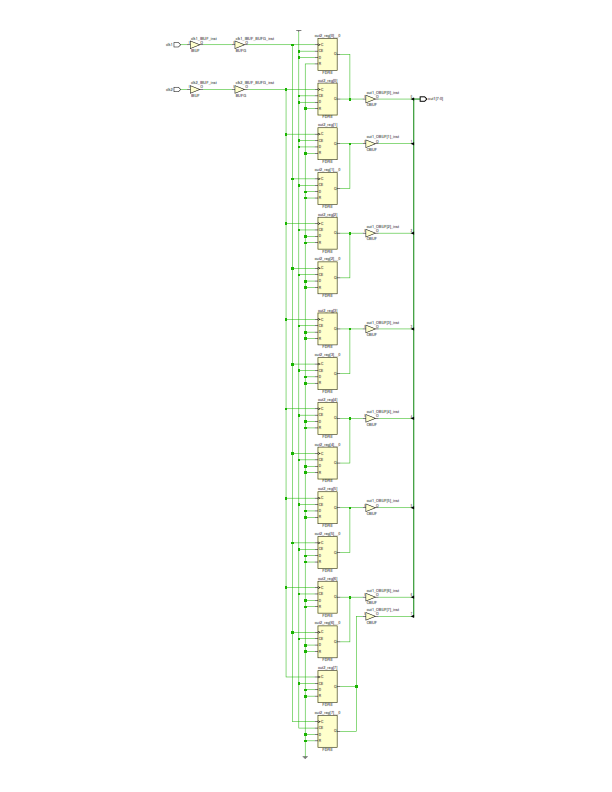
\includegraphics[height=12cm]{src/p3/schematic.png}\\

\textit{In vivado synthesis we have errors for multi deriven signals.}

%------- P4

\section{Problem 4}
\subsection{Part 1}
\inputminted{vhdl}{src/p4-1-2/p4-1.vhd}
\subsection{Part 2}
\inputminted{vhdl}{src/p4-1-2/p4-2.vhd}
\subsection{Part 3}
\inputminted{vhdl}{src/p4-3/p4-3.vhd}
\subsection{Part 4}
\inputminted{vhdl}{src/p4-4/p4-4.vhd}
\subsection{Part 5}
\inputminted{vhdl}{src/p4-5/p4-5.vhd}

%------- P5

\section{Problem 5}
\subsection{Part 1}
\begin{center}
	\begin{tabular}{c | c | c || r}
		A & B & C & F \\
		\hline
		0 & 0 & 0 & 0 \\
		\hline
		0 & 0 & 1 & 1 \\
		\hline
		0 & 1 & 0 & 0 \\
		\hline
		0 & 1 & 1 & 1 \\
		\hline
		1 & 0 & 0 & 0 \\
		\hline
		1 & 0 & 1 & 0 \\
		\hline
		1 & 1 & 0 & 1 \\
		\hline
		1 & 1 & 1 & 1 \\
		\hline
	\end{tabular}
\end{center}
\subsection{Part 2}
\inputminted{vhdl}{src/p5-2/p5-2.vhd}

\end{document}
